\documentclass[11pt]{article}

\usepackage{pdfpages}
\usepackage{hyperref}
\usepackage{enumerate}
\usepackage{listings}
\usepackage{float}

\renewcommand*\ttdefault{lmtt}
\renewcommand*\sfdefault{lmss}
\renewcommand{\familydefault}{\sfdefault}

\begin{document}

\author{Group 8}
\title{Laboratory Work 1}
\maketitle

\section{Assignment 1}

\begin{figure}[H]
  \centering
   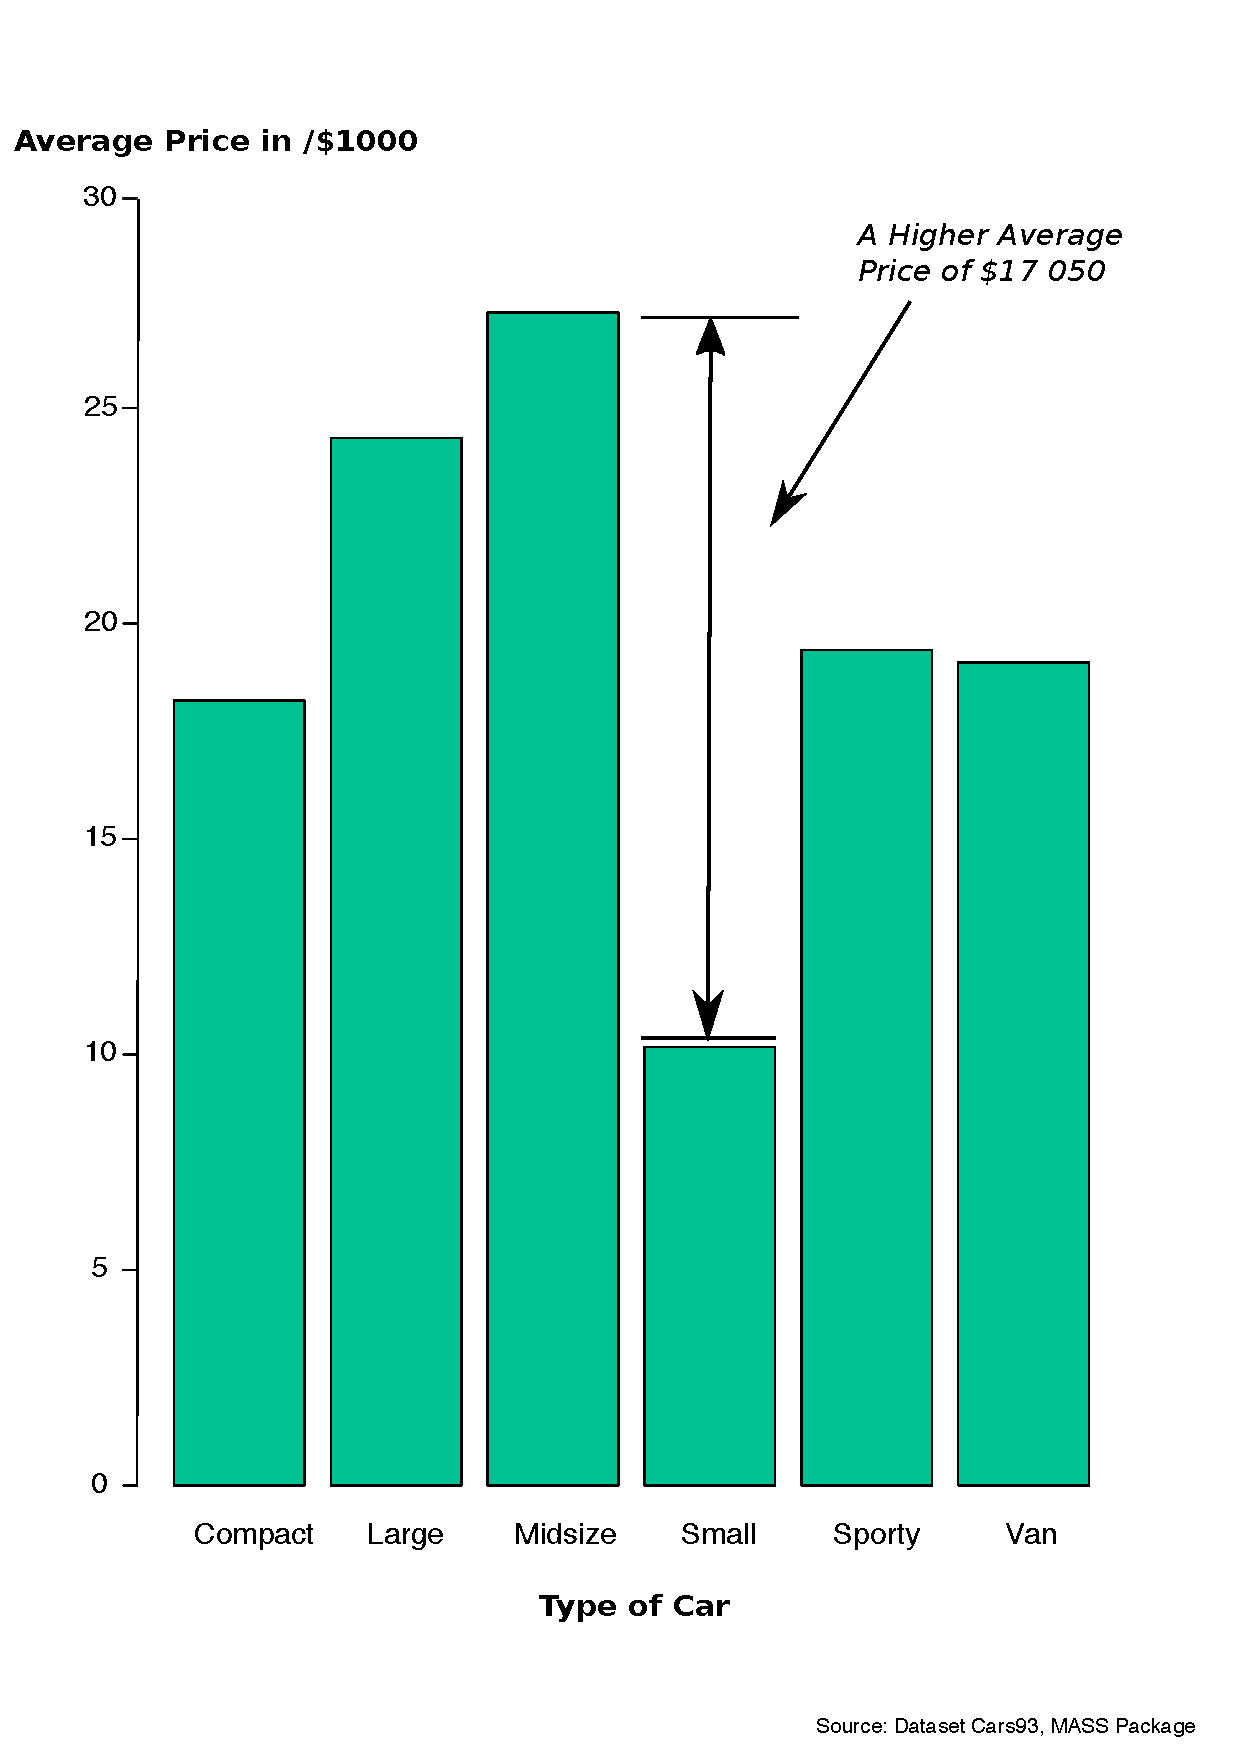
\includegraphics[scale=0.4]{Assignment_1.pdf}
   \caption{The Average Car Price for each type of Car}
\end{figure}


\section{Assignment 2}

% TODO: Adjust the picture so that it centres in the page

\begin{figure}[H]
  \centering
  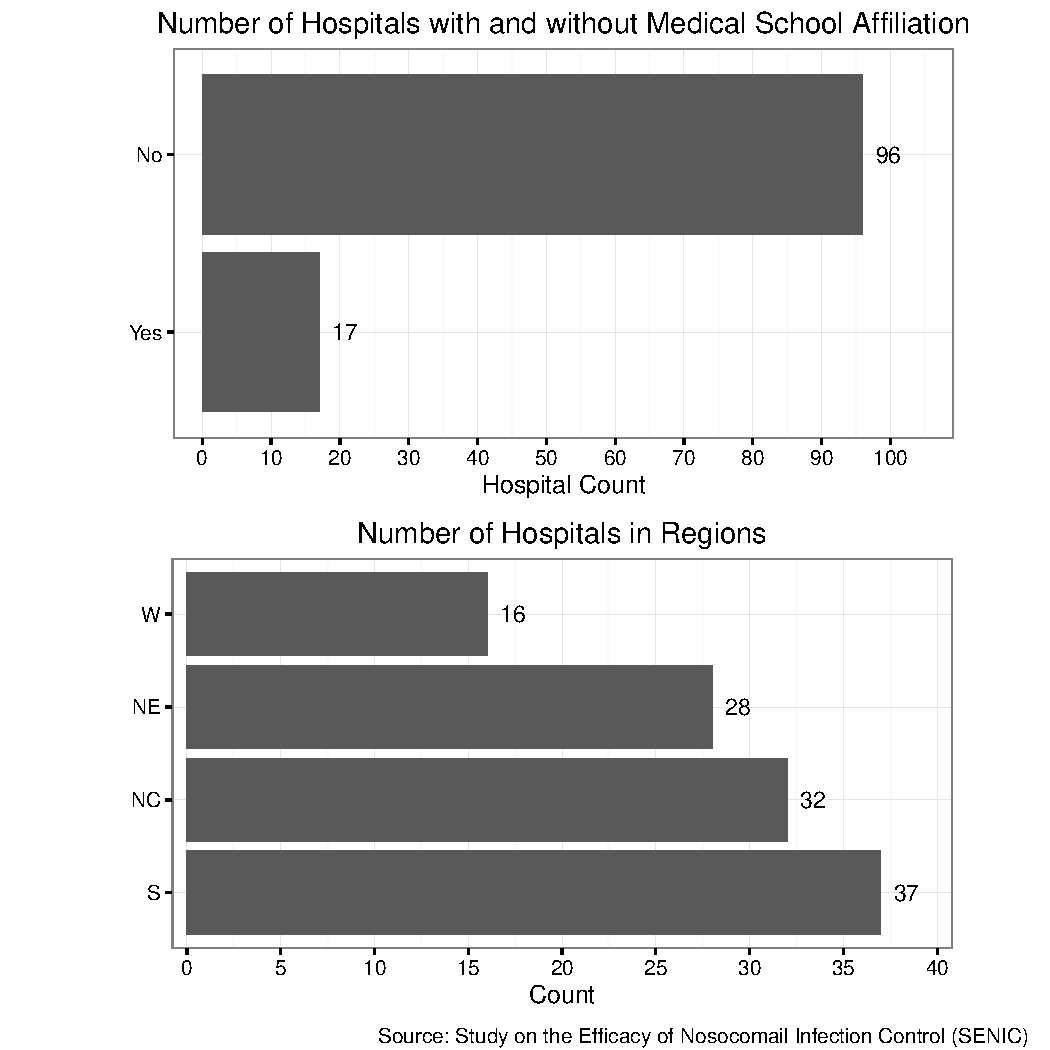
\includegraphics[scale=0.8]{qualitative_vars.pdf}
  \caption{Count of observations of the two
    qualitative variables}
  \label{fig:qualivars}
\end{figure}

There are only two qualitative variables among all: the Medical School
Affiliation (X7) and Region (X8). \autoref{fig:qualivars} is the combined
chart requested.

We can observe from \autoref{fig:qualivars} that
\begin{enumerate}
\item
  Only a few hospitals have affiliation with medical schools.
\item
  The number of hospital in a region varies a lot across regions. This
  does not tell us anything meaningful, however, unless this count is
  normalized by the population size of each regions. So if this is an
  real analysis, the next step may be to construct a graph of the ratio
  'hospital number/population-size', or even better
  'number of bed/population-size'.
\end{enumerate}



\begin{figure}[H]
  \centering
  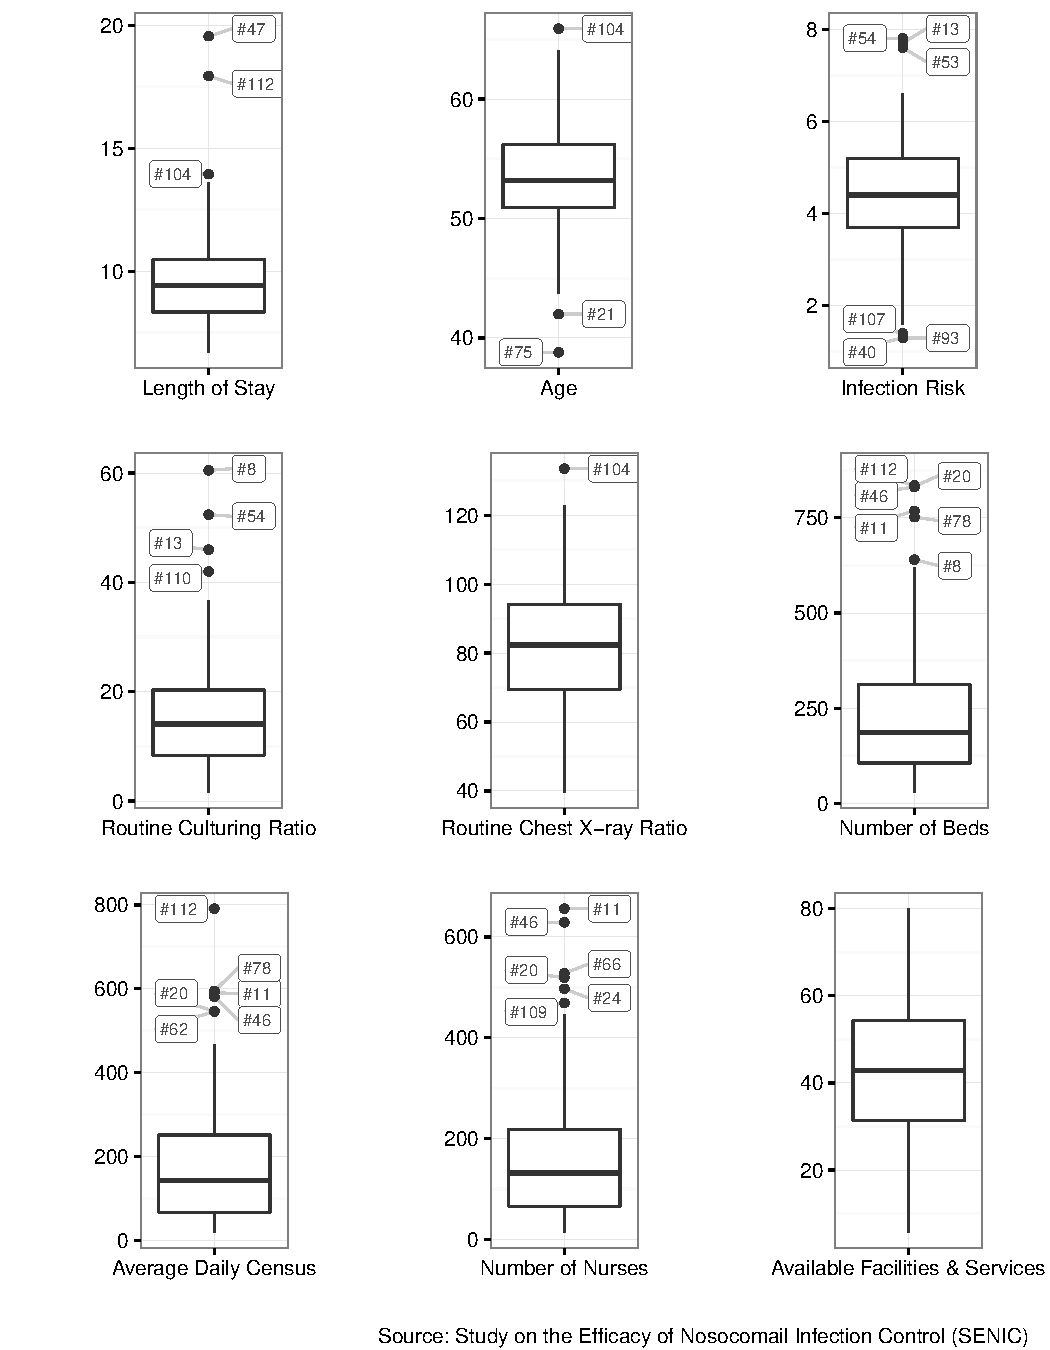
\includegraphics[scale=0.8]{quantitative_vars.pdf}
  \caption{Combined plot of all quantitative variables}\label{fig:quantvars}
\end{figure}

The quantitative variables are plotted in box plots in \autoref{fig:quantvars}.

The following are some observations:
\begin{enumerate}
\item
  Average length of stay varies among the hospitals from less than five days to
  near 20 days. This suggest that some hospitals does not have bed or service of
  taking many long-staying patients.
\item
  Both number of nurses, average daily census and number of beds ranges from
  several dozens to several hundreds. They also shares many outliers. This suggest
  some hospitals are having many staying patients and some hospitals doesn't take
  in many staying patients at all.
\item
  Hospital \#104 outlies in both length of stay and average age of patient. It
  seems that this hospital probably has a geriatric or paliative care service.
  Its outlying in routine chest X-ray ratio may be related to this as well.
\item
  Hospital \#13 and \#54 outlies together in both infection risk and routine culturing
  ratio. Both intuition and this coincidence leads us to suspect there is corelation
  between culturing and infection. Ploting them in a scatter plot may help us find
  this out.
\end{enumerate}


\section{Assignment 3}

\begin{figure}[H]
  \centering
   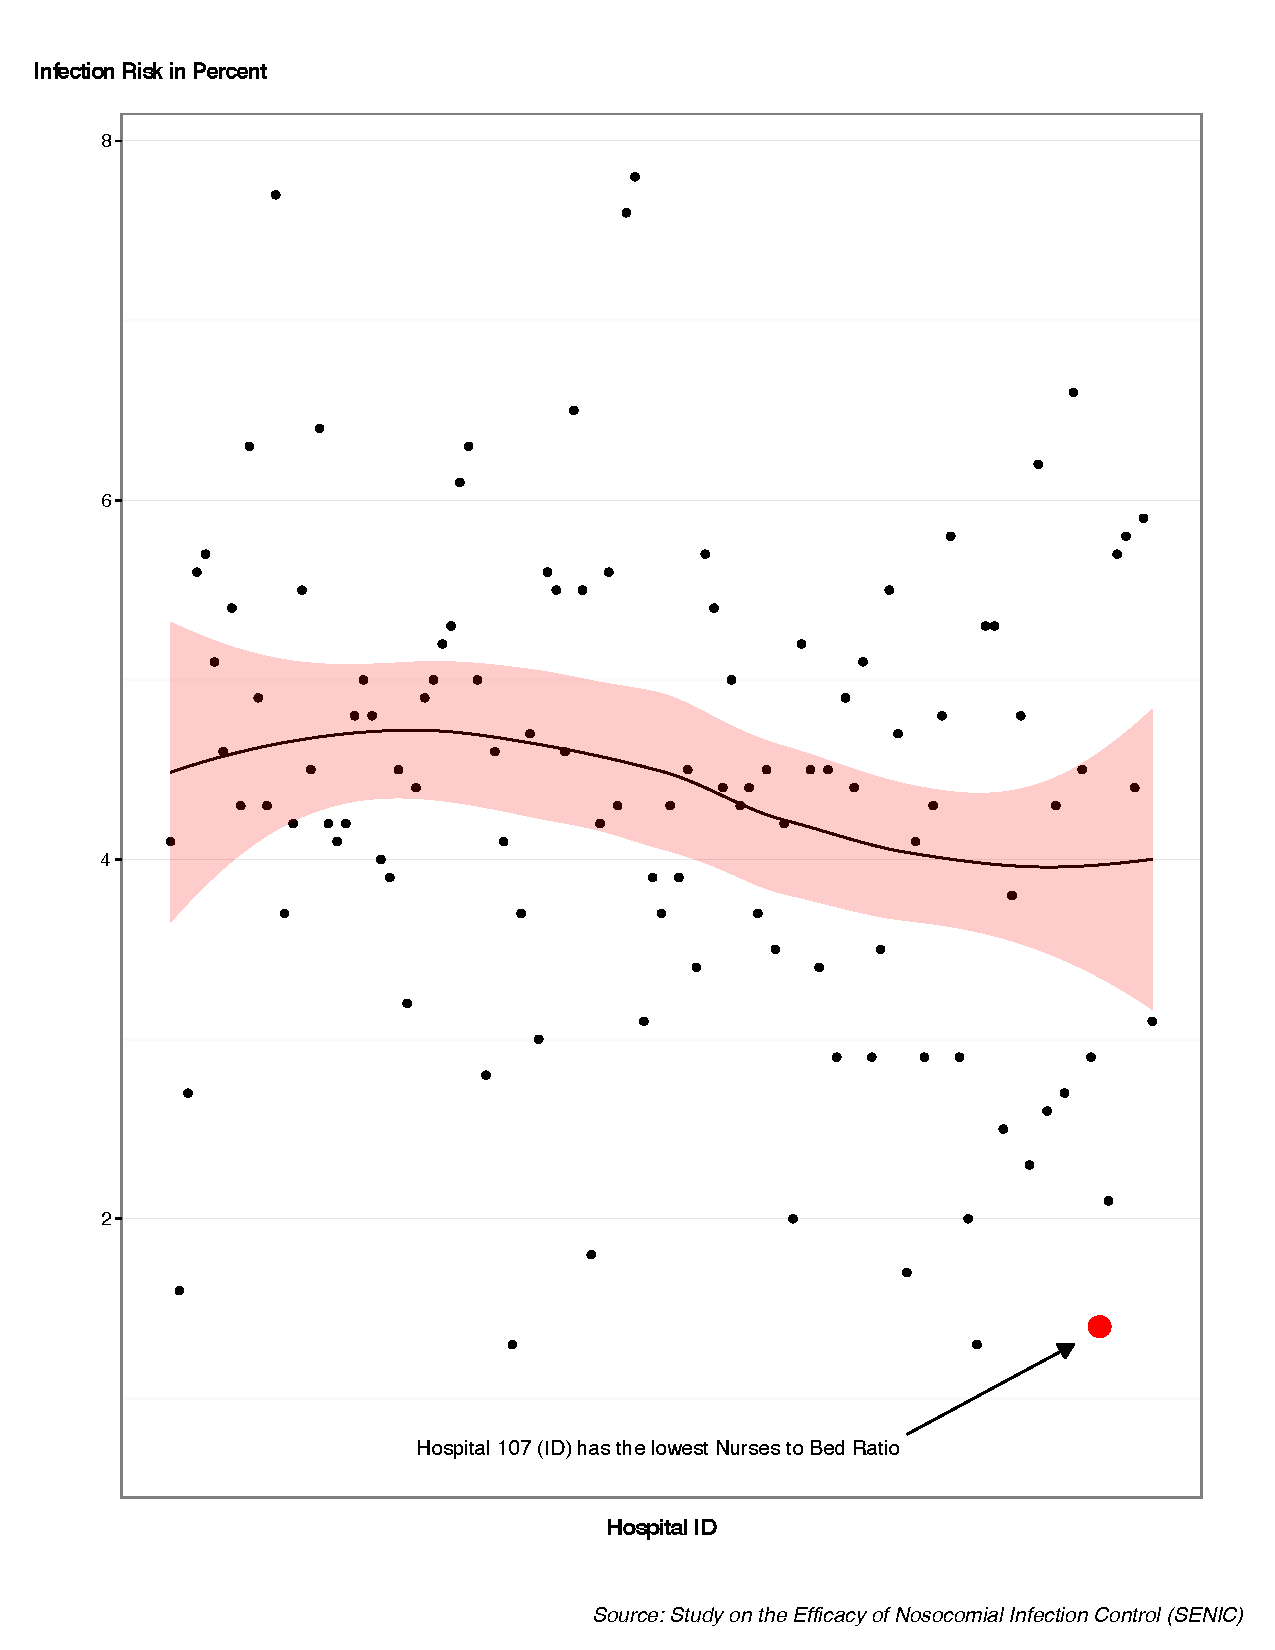
\includegraphics[scale=0.5]{Assignment_3.pdf}
\end{figure}




\end{document}

